\subsection{Основы финансово-экономического анализа и планирования}
	
	\subsubsection{Аннотация}

		Курс <<Основы финансово-экономического анализа и планирования>> получил в основном положительные оценки.

		Руководствуясь результатами опроса, Совет студентов и аспирантов ФРКТ выдвигает следующие идеи по улучшению данного курса:
		\begin{enumerate}
			\item пересмотреть содержание курса, чтобы материал был более детальным и полезным для студентов;
			\item провести пересмотр тестовых вопросов, чтобы исключить ошибки и некорректные формулировки;
			\item добавить разбор реальных экономических событий, чтобы повысить интерес и практическую пользу для обучающихся.
		\end{enumerate}


	\subsubsection{Общий отзыв студентов о курсе}

		\begin{figure}[H]
			\centering
			\begin{subfigure}[b]{0.45\textwidth}
				\centering
				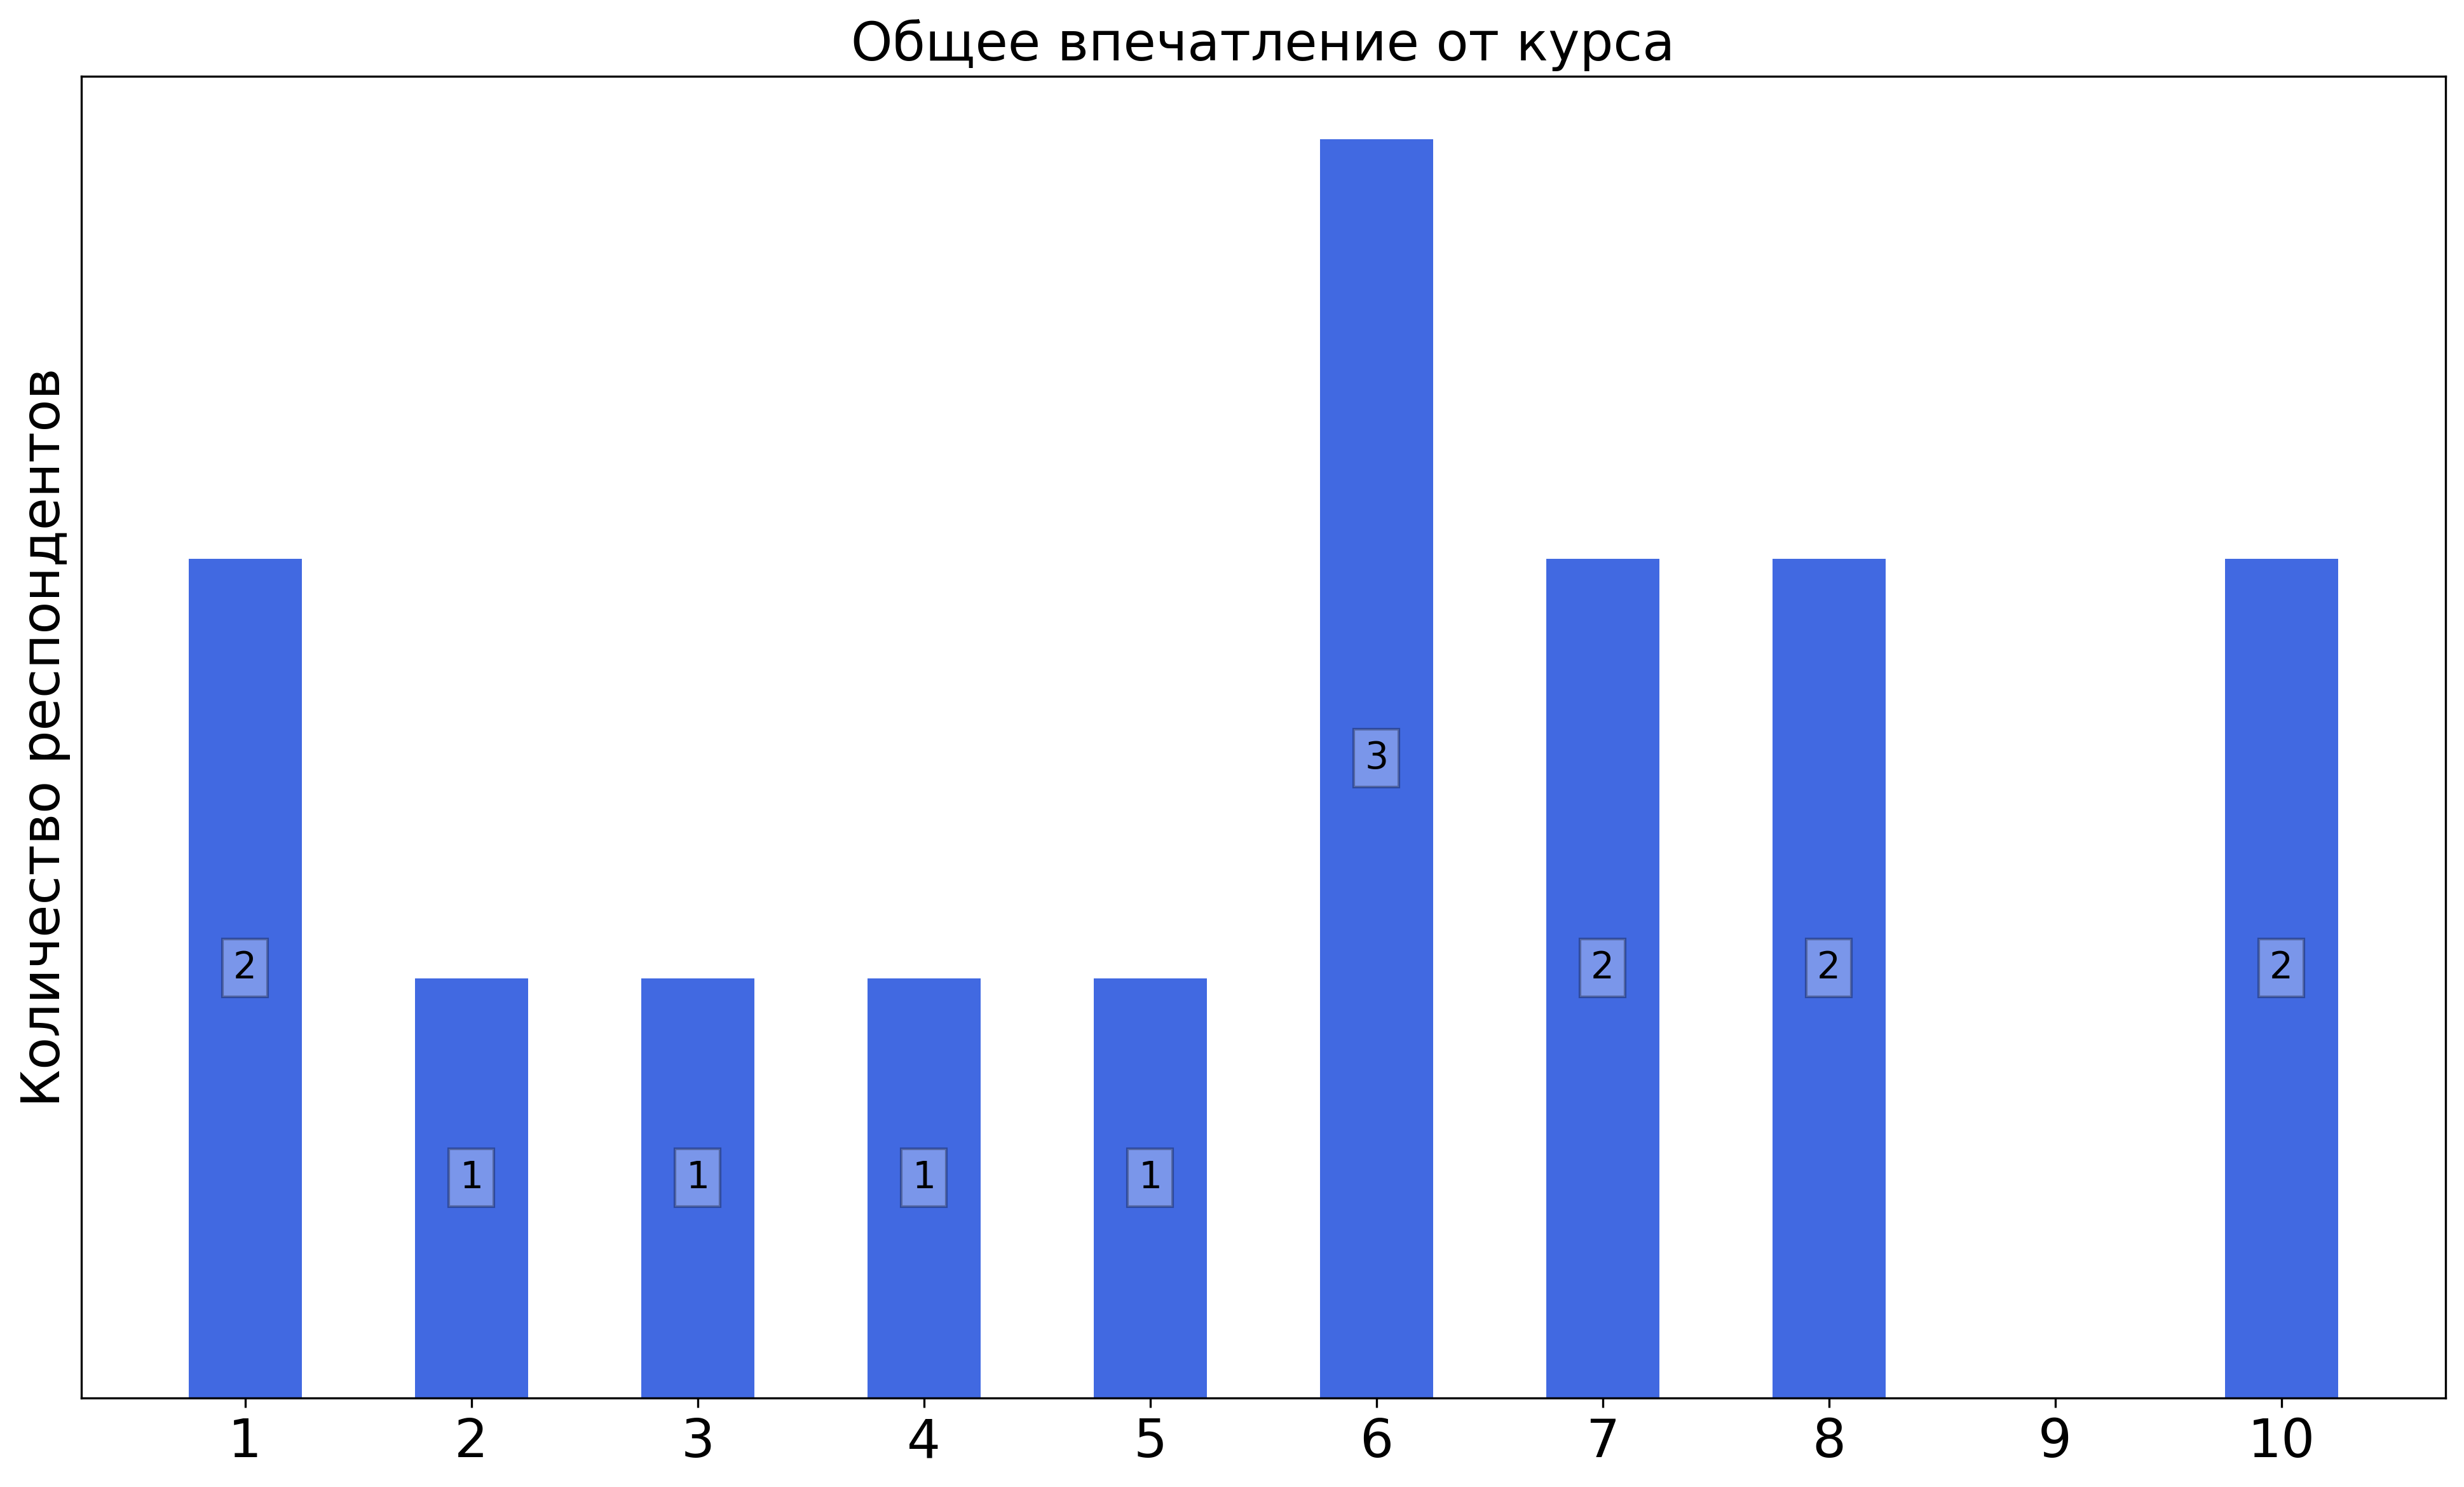
\includegraphics[width=\textwidth]{images/4 course/Основы финансово-экономического анализа и планирования/general-0.png}
			\end{subfigure}
		\end{figure}

	\subsubsection{Материалы, использумые респондентами при изучении курса}

		\begin{figure}[H]
			\centering
			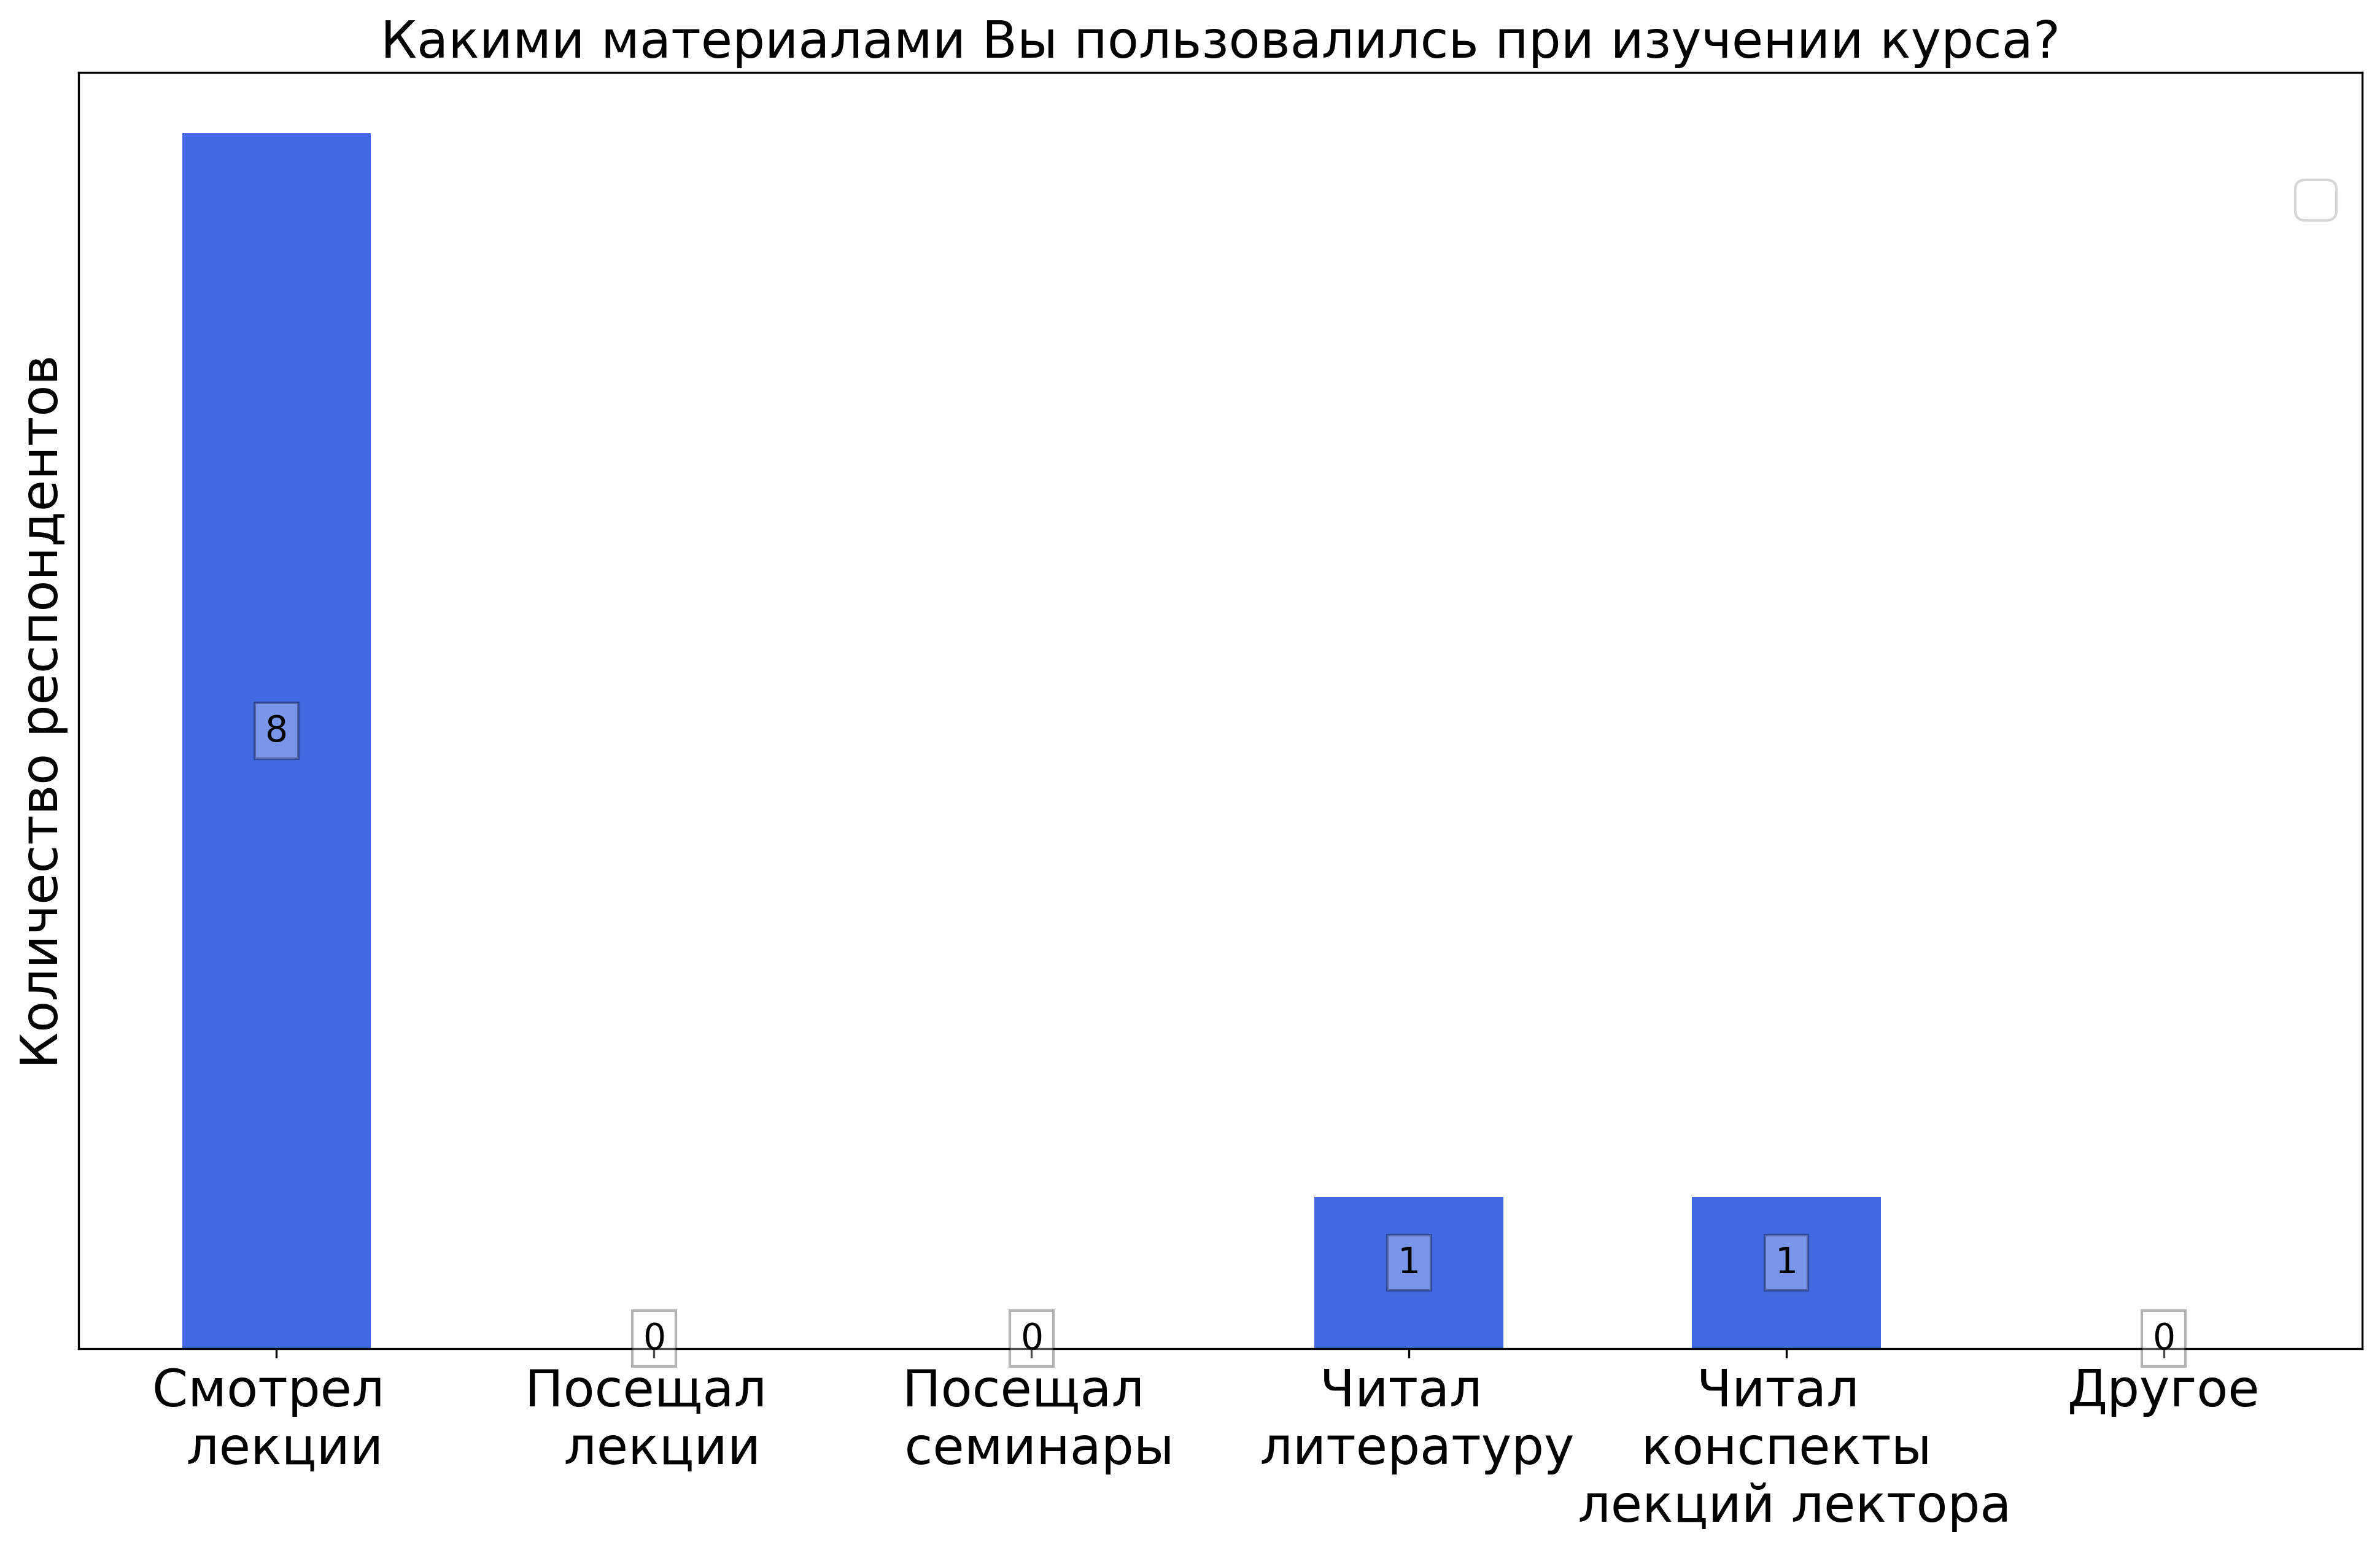
\includegraphics[width = 0.45\textwidth]{images/4 course/Основы финансово-экономического анализа и планирования/materials.png}
		\end{figure}


	\subsubsection{Отзыв студентов о лекциях. Лектор: Старостин Е.А.}

		\begin{figure}[H]
			\centering
            \begin{subfigure}[b]{0.45\textwidth}
				\centering
				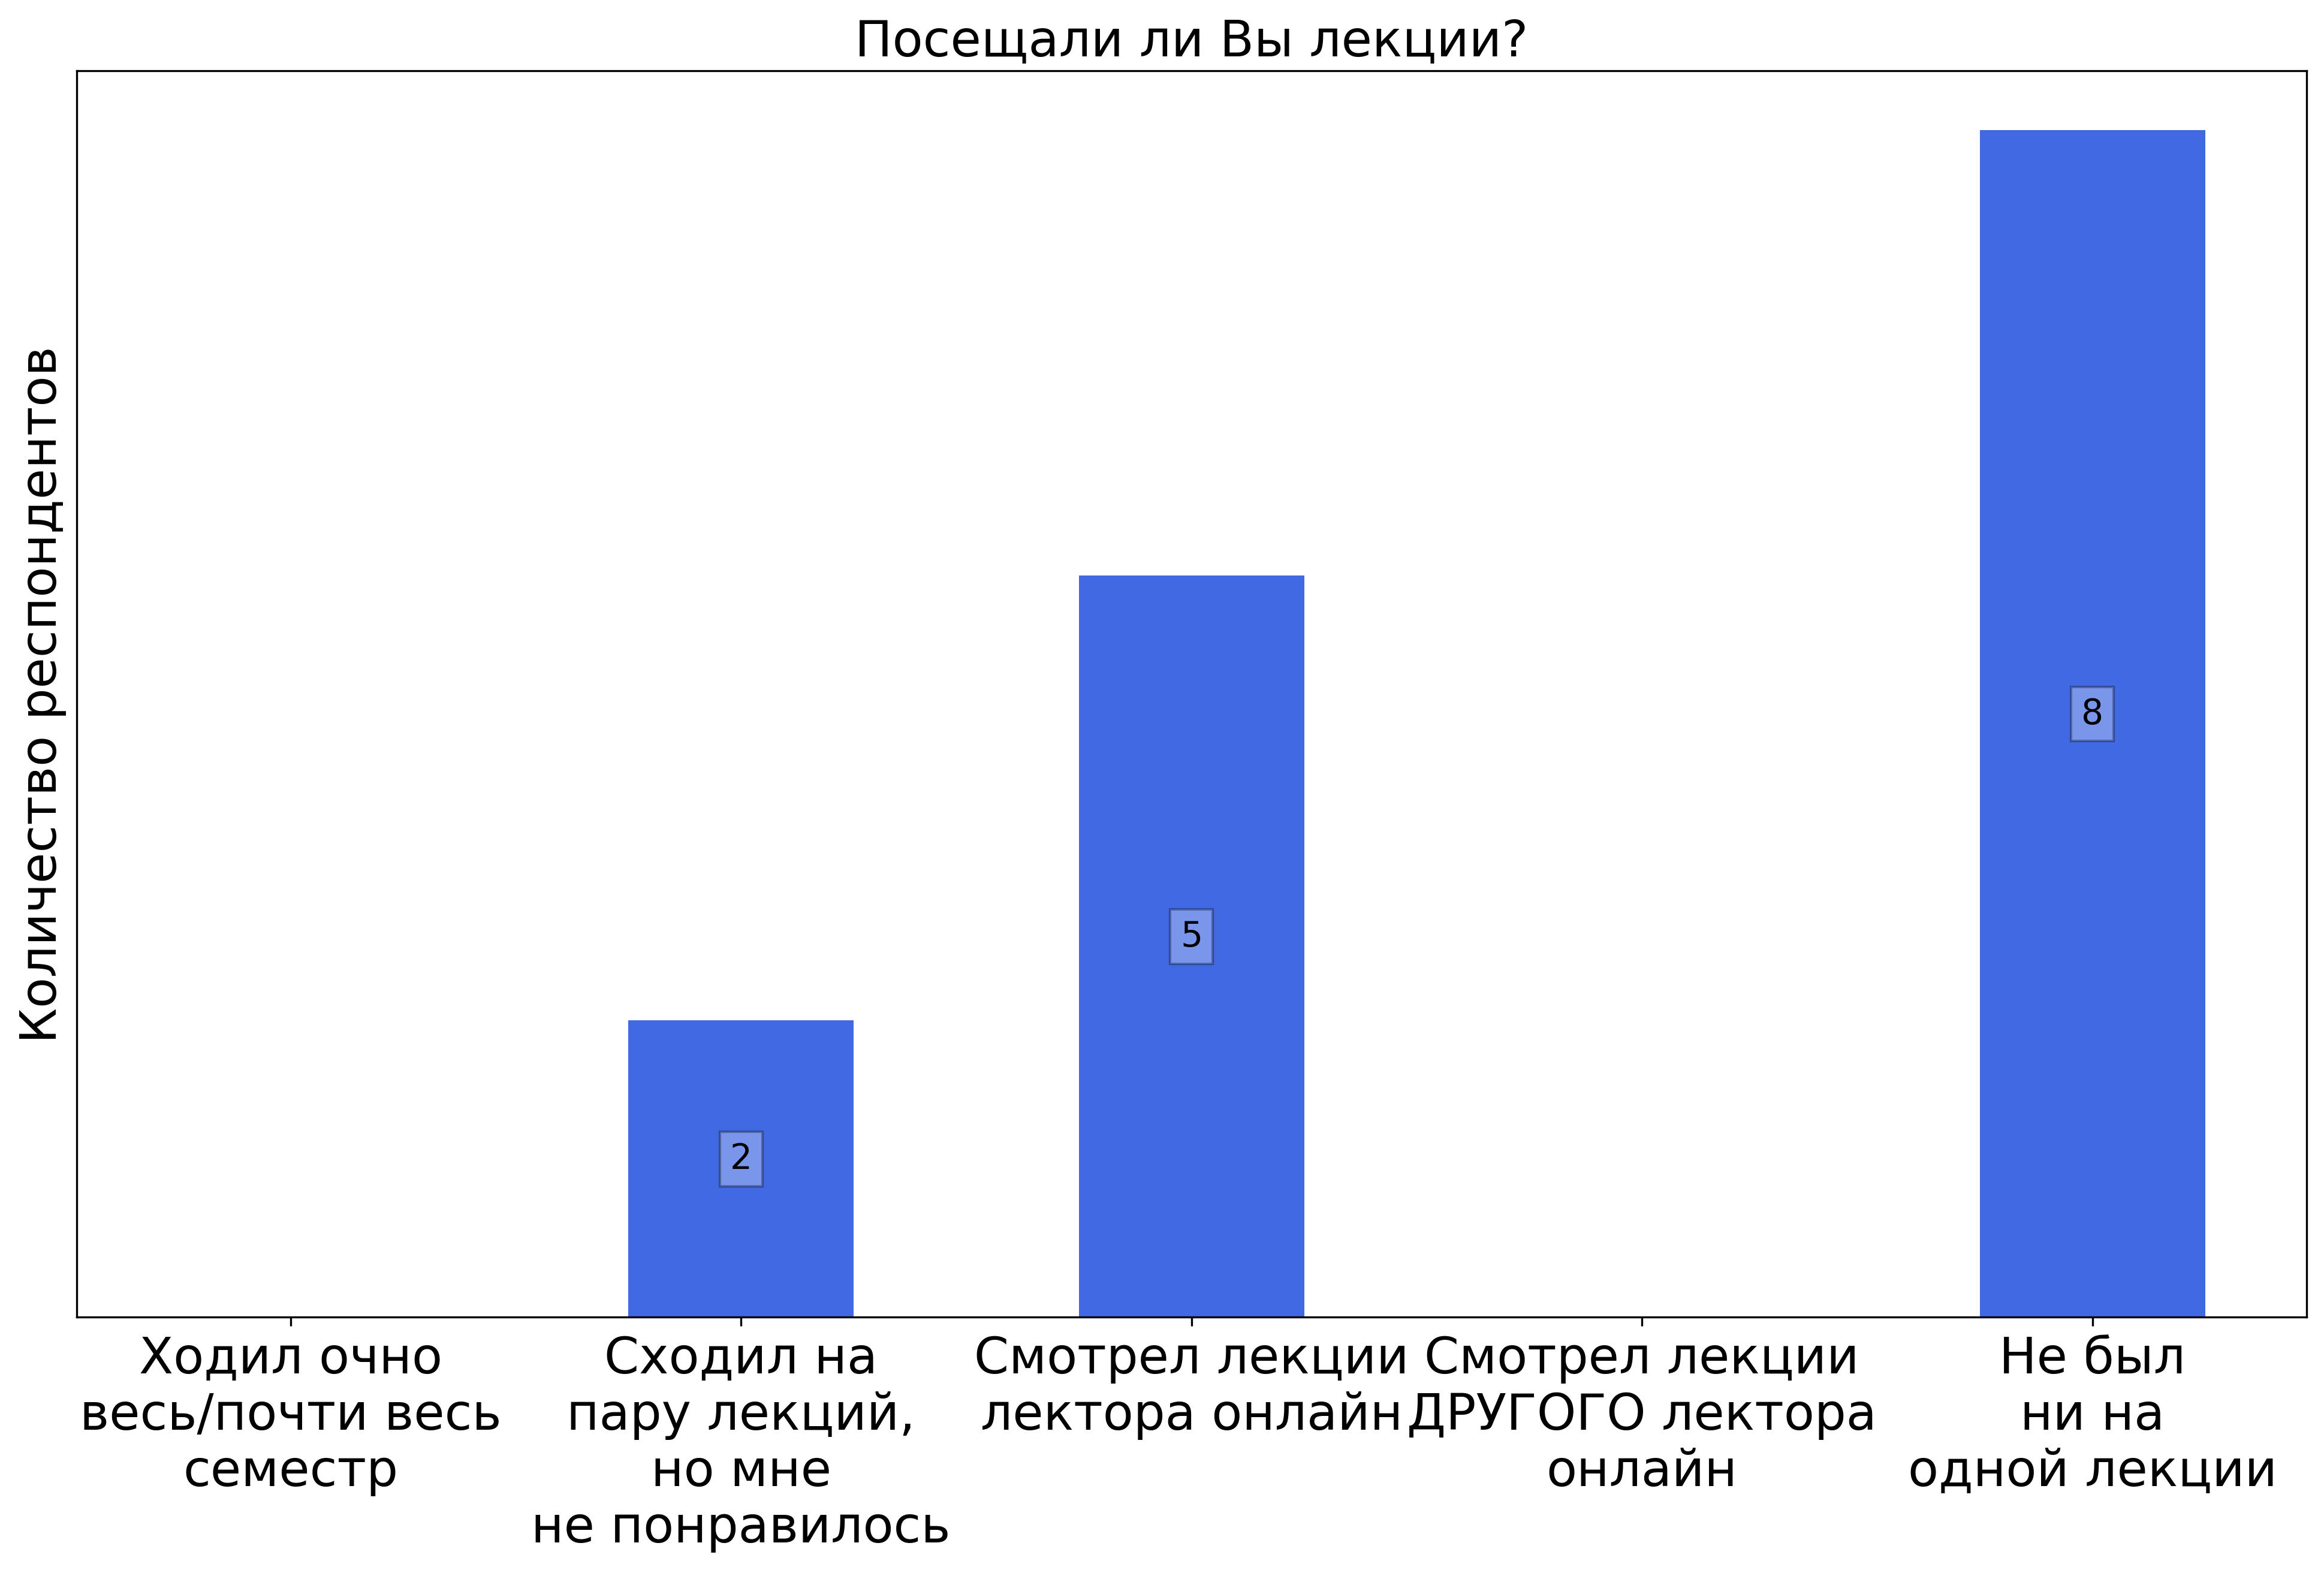
\includegraphics[width=\textwidth]{images/4 course/Основы финансово-экономического анализа и планирования/lecturer-questions-Старостин Е.А.-0.png}
			\end{subfigure}
			\begin{subfigure}[b]{0.45\textwidth}
				\centering
				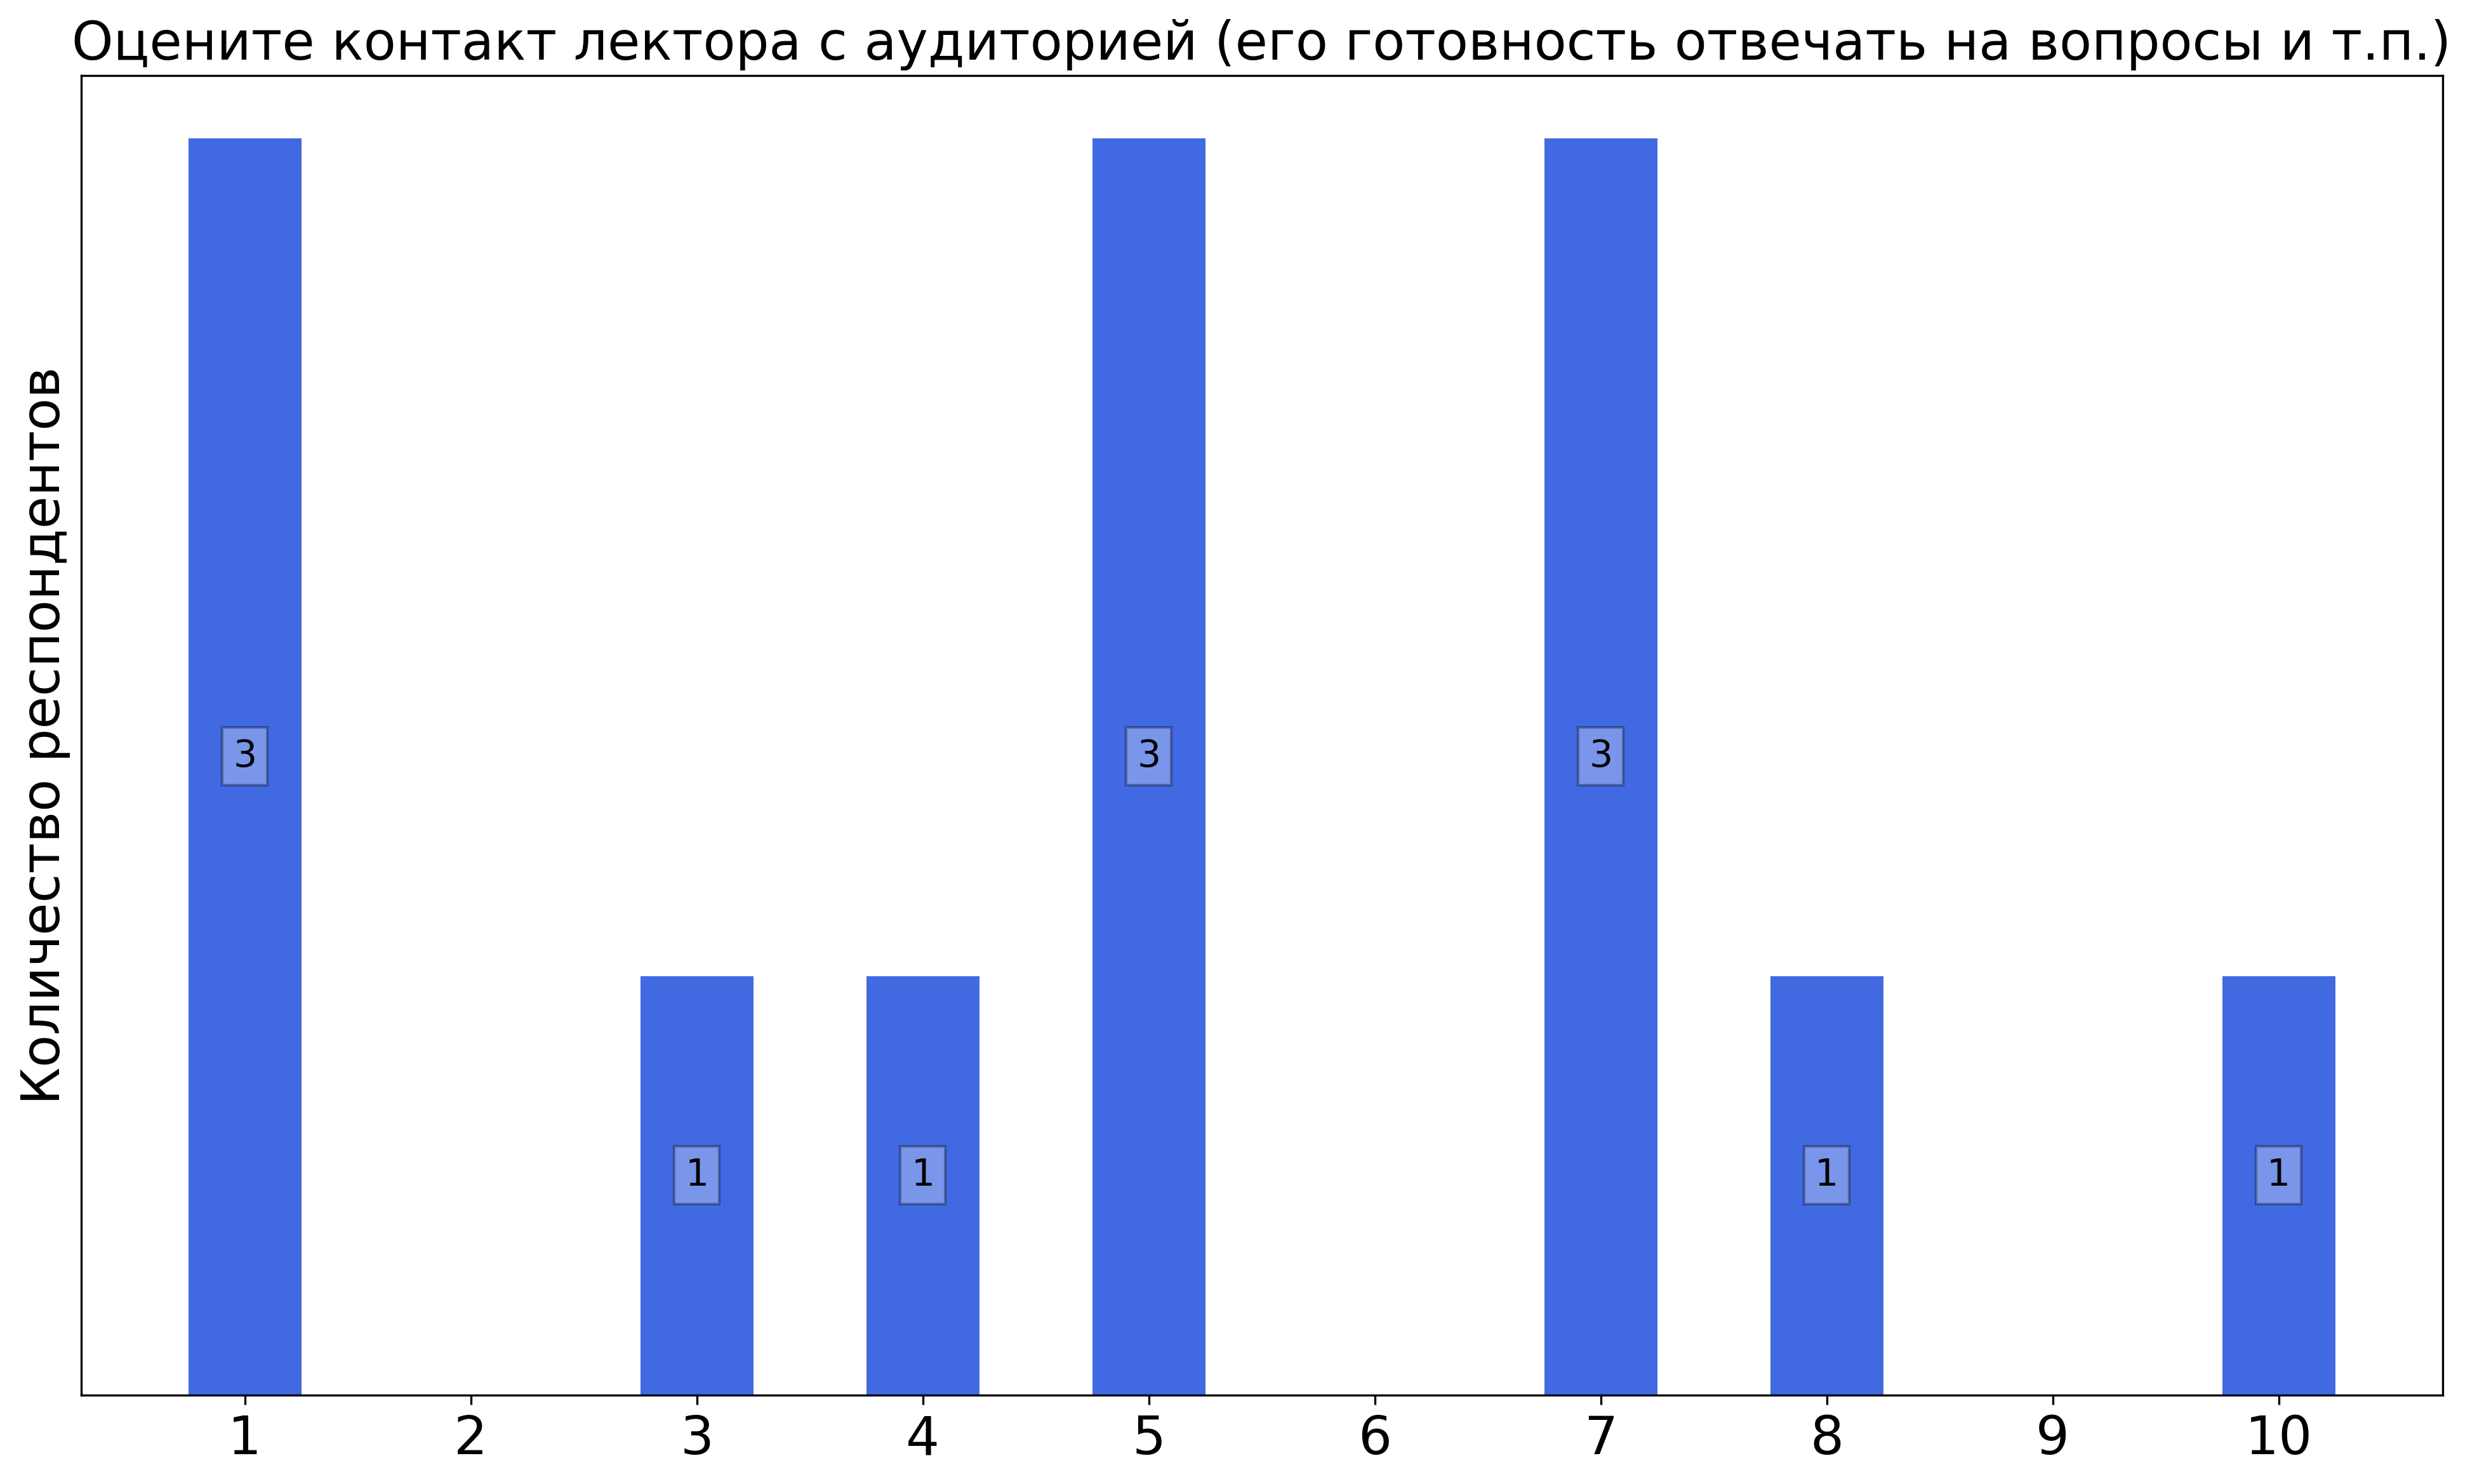
\includegraphics[width=\textwidth]{images/4 course/Основы финансово-экономического анализа и планирования/lecturer-marks-Старостин Е.А.-0.png}
			\end{subfigure}
			\begin{subfigure}[b]{0.45\textwidth}
				\centering
				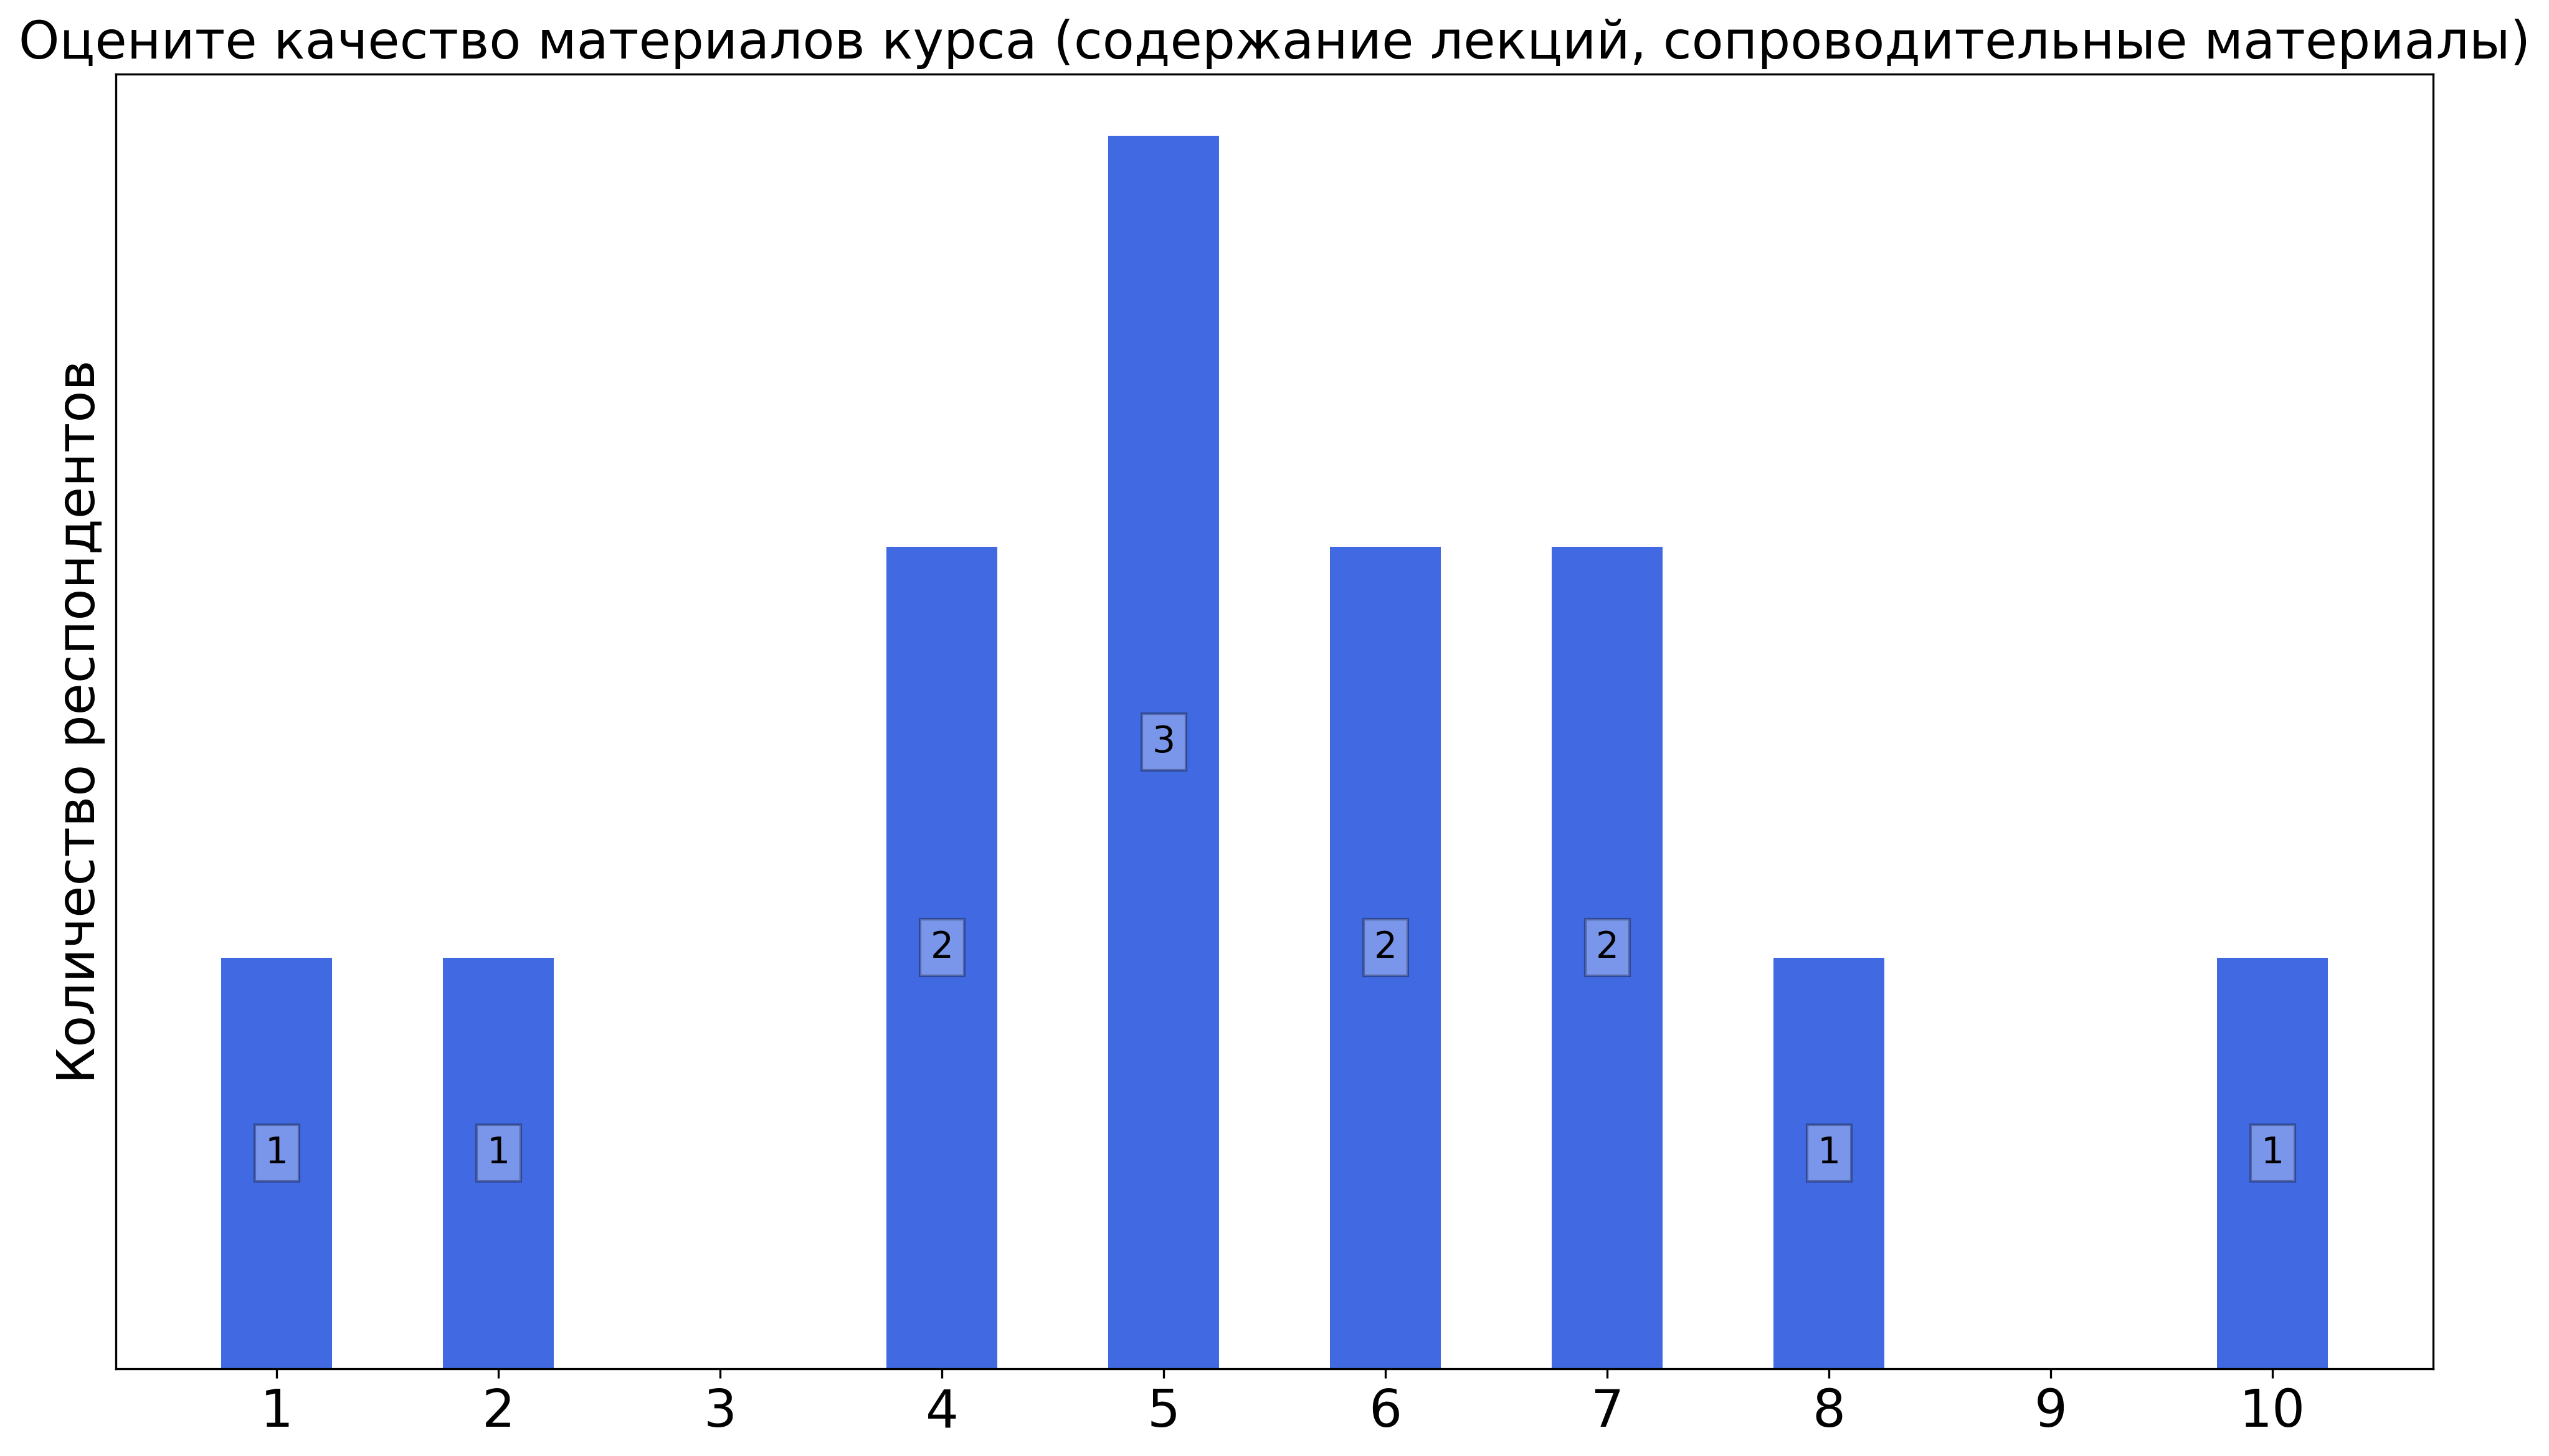
\includegraphics[width=\textwidth]{images/4 course/Основы финансово-экономического анализа и планирования/lecturer-marks-Старостин Е.А.-1.png}
			\end{subfigure}
			\begin{subfigure}[b]{0.45\textwidth}
				\centering
				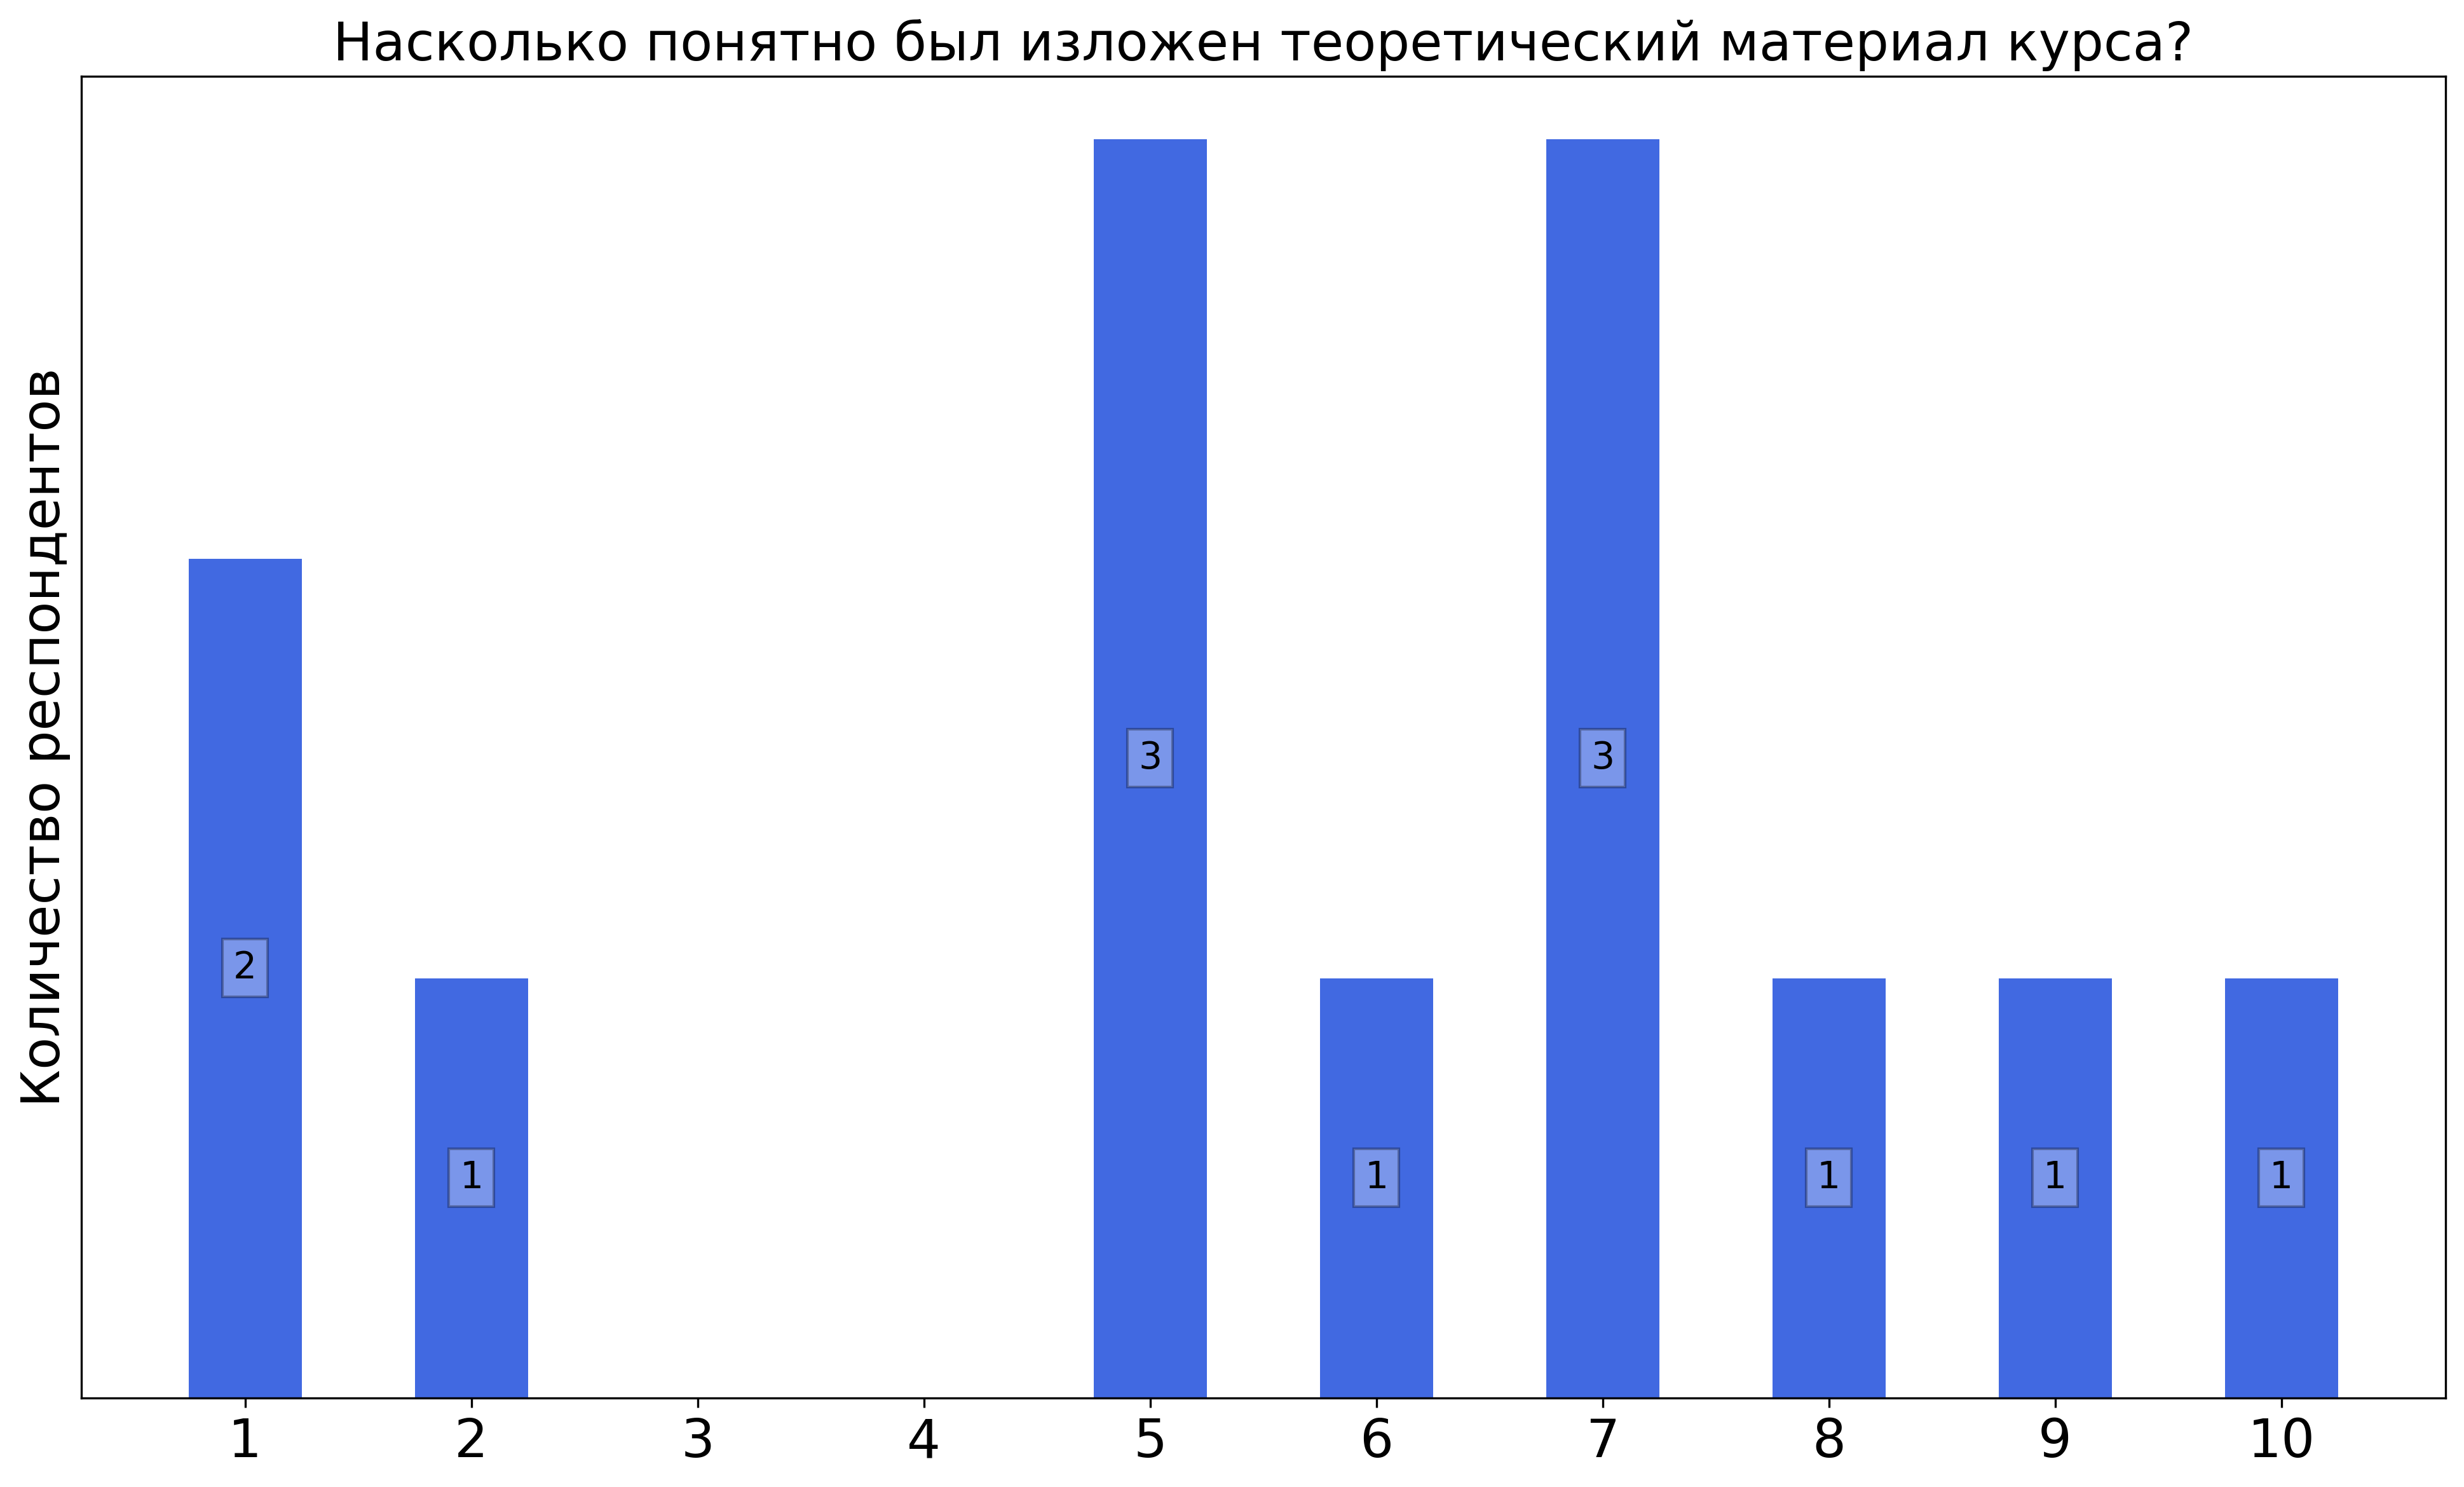
\includegraphics[width=\textwidth]{images/4 course/Основы финансово-экономического анализа и планирования/lecturer-marks-Старостин Е.А.-2.png}
			\end{subfigure}	
			\begin{subfigure}[b]{0.45\textwidth}
				\centering
				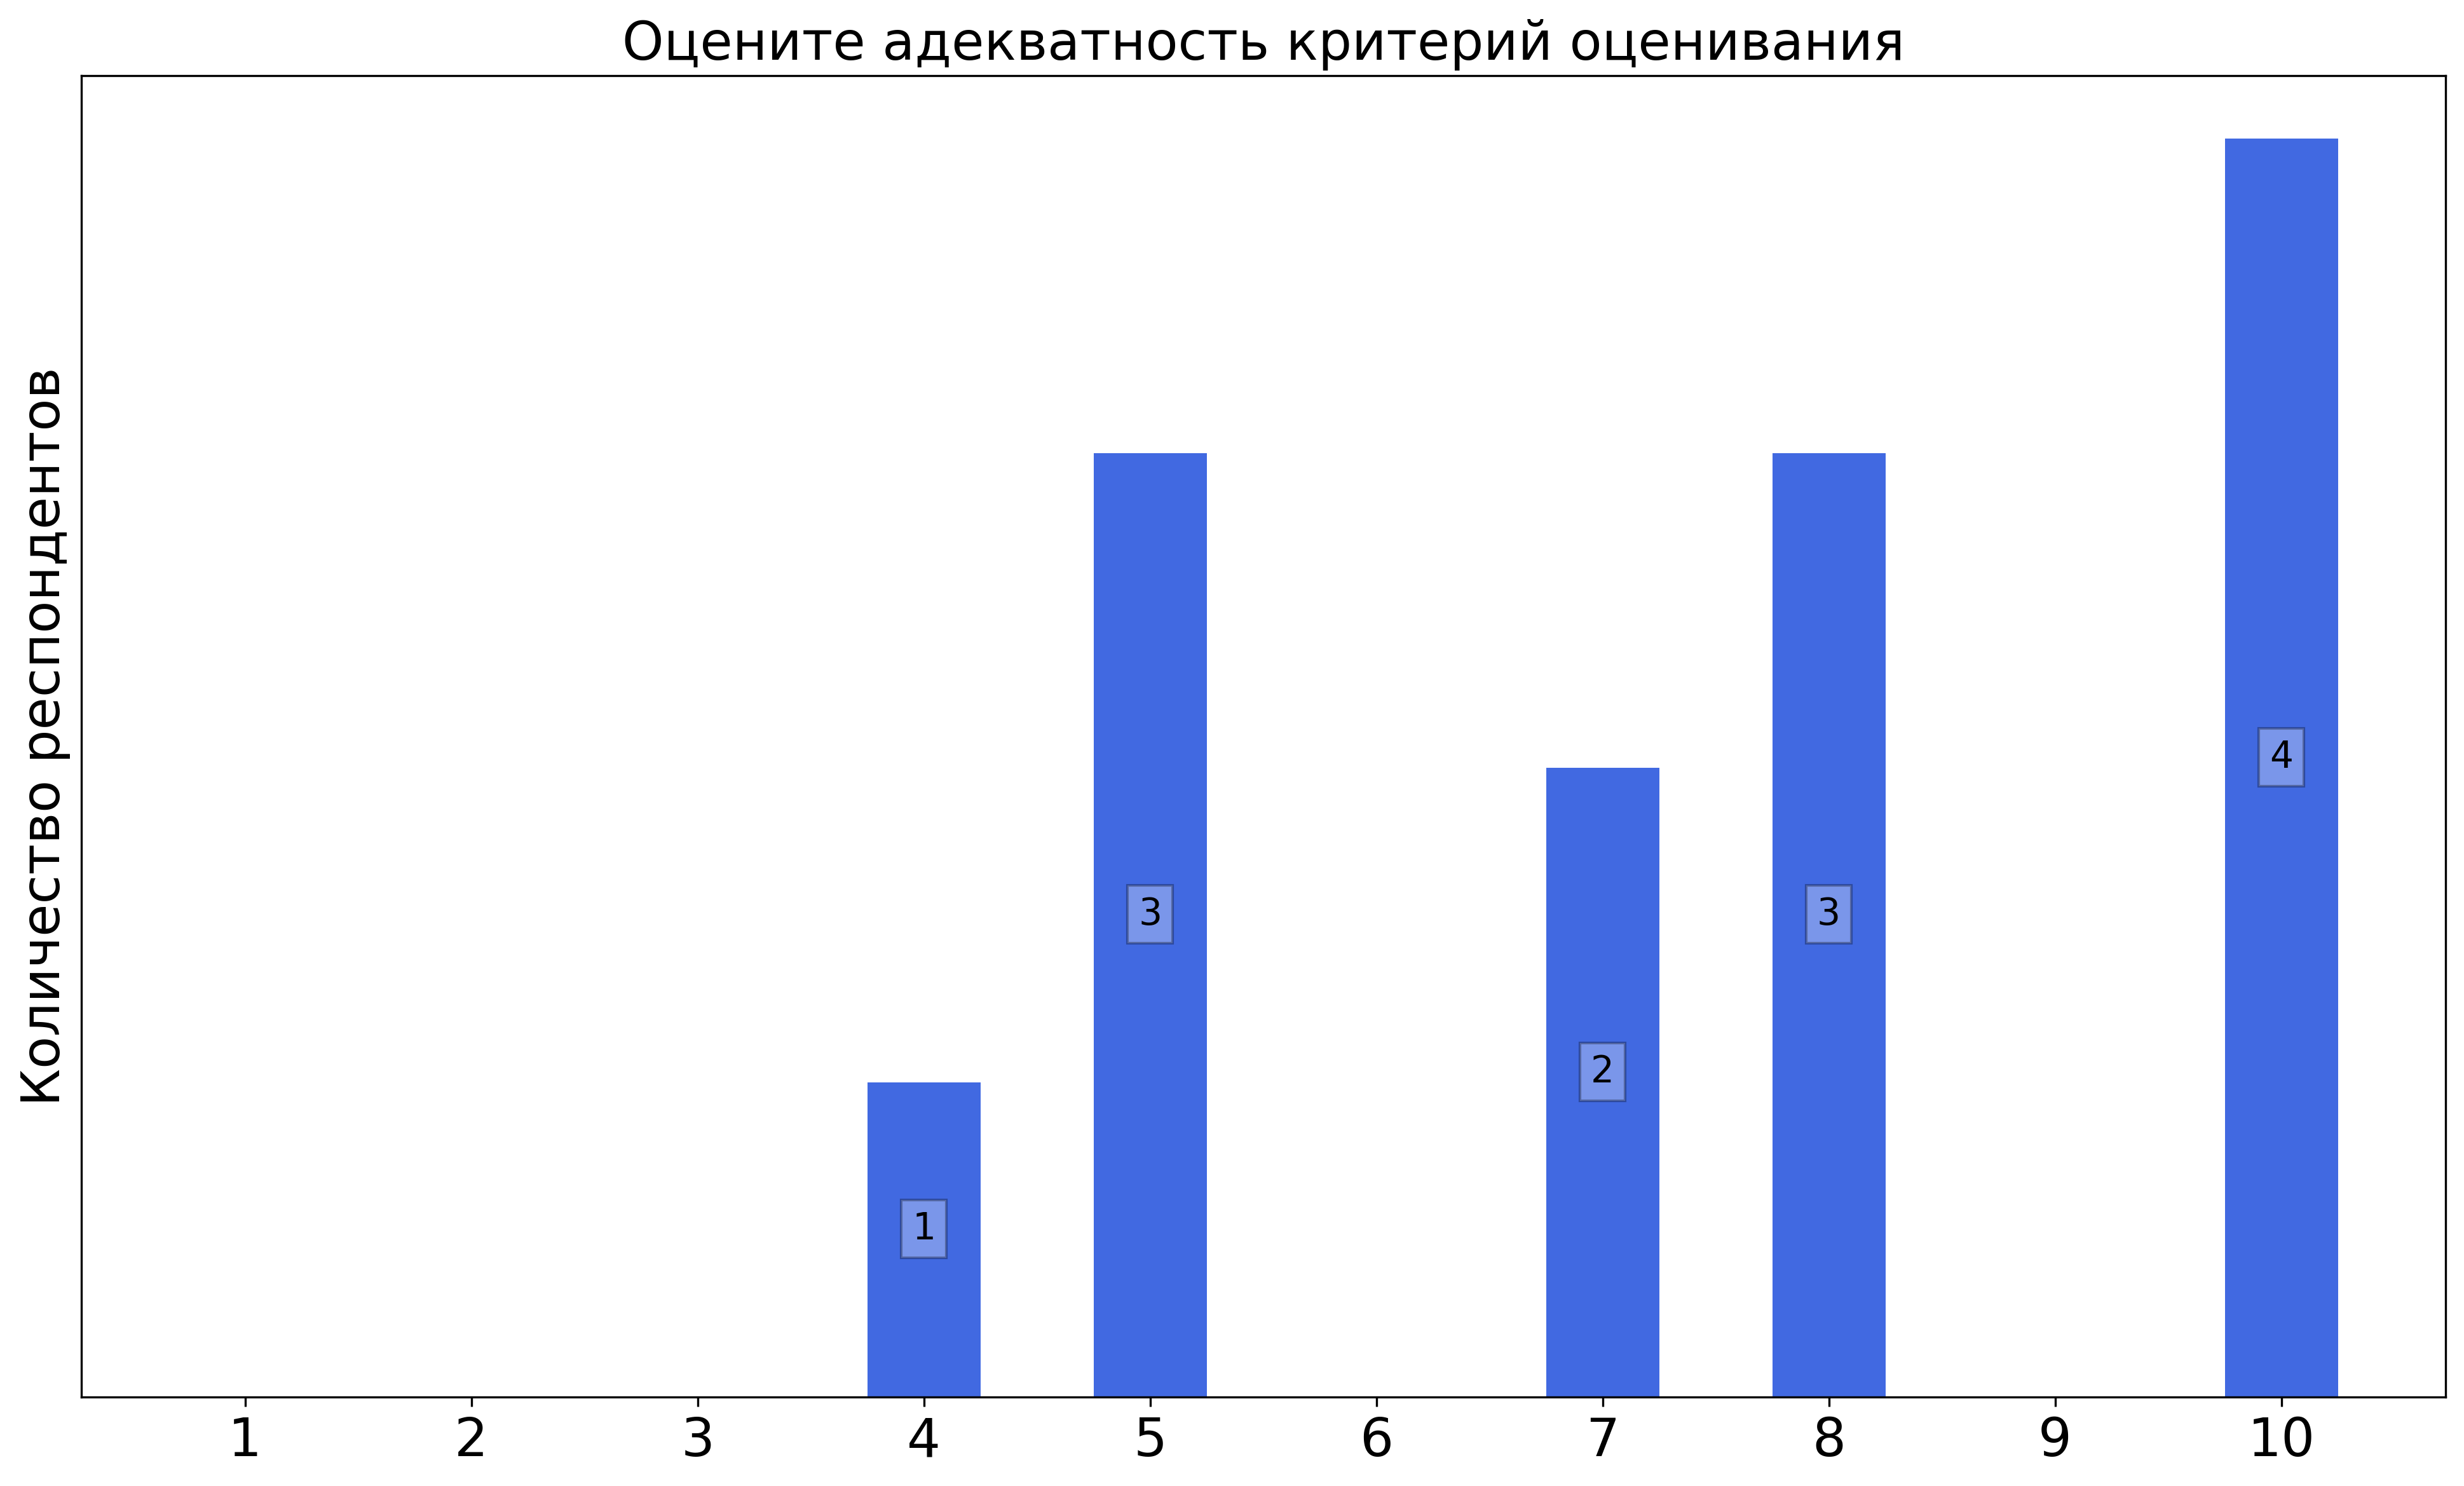
\includegraphics[width=\textwidth]{images/4 course/Основы финансово-экономического анализа и планирования/lecturer-marks-Старостин Е.А.-3.png}
			\end{subfigure}
			\caption{Оценки респондентов о качестве преподавания лекций по курсу <<Основы финансово-экономического анализа и планирования>>}
		\end{figure}

		\textbf{Комментарии студентов о лекциях\protect\footnote{сохранены оригинальные орфография и пунктуация}}
            \begin{commentbox} 
                Записанные видео ролики по которым надо делать онлайн тестики - не могу назвать предметом. 
        
                Материал изложен поверхностно, задачи тяжело с ним решать.  
            \end{commentbox} 
        
            \begin{commentbox} 
                Курс на лмс (что плюс), вопросы не корректны 
            \end{commentbox} 
        
    
    \subsubsection{Прочие комментарии и предложения по улучшению курса}
        \begin{commentbox}
            Тесты с ошибками были. И рассылку от каждого сообщения в форуме лмс стоит убрать. 
        \end{commentbox}

        \begin{commentbox}
            Без понятия, для чего этот курс в принципе нужен
        \end{commentbox}

        \begin{commentbox}
            Курс не особо создан как нужный и интересный, но зато он сделан так чтоб не было проблем с его закрытием. Можно было бы создать что то более актуальное и интересное в идеале, но и ботать экономику на уровне экономистов нам не очень востребовано. Так что было бы полезна прикладная сторона вопроса, для нас как для пользователей вкладов, инвестиций и тд. Было бы полезно если бы какие то актуальные события экономики разбирались. Но я понимаю что обновлять программу каждый год очень накладно и надо искать компромисс.
        \end{commentbox}

        \begin{commentbox}
            Курс работает как курс для галочки, пусть так и будет
        \end{commentbox}

        \begin{commentbox}
            Выделять больший промежуток времени на выполнение тестов на lms или давать возможность переписать его в течение семестра, если пропуск был уважительным. Делать какое-то напоминание о тестах тоже было бы неплохо 
        \end{commentbox}